\documentclass[12pt,letterpaper]{article}
\usepackage{amsmath, amssymb, amsthm}
\newtheorem{theorem}{Proposition}
\theoremstyle{remark}
\newtheorem*{remark}{Remark}
\usepackage{graphicx}
\usepackage{setspace}
\usepackage{amsmath, amssymb, amsthm}
%\newtheorem{theorem}{Proposition}
\theoremstyle{remark}
%\newtheorem*{remark}{Remark}
\usepackage[T1]{fontenc}
\usepackage{setspace}
\usepackage{pdflscape}
\usepackage{booktabs, threeparttable, tabularx, makecell, siunitx}
\DeclareMathOperator*{\rint}{\ThisStyle{\rotatebox{15}{$\SavedStyle\!\int\!$}}}
\usepackage{indentfirst}
\usepackage{xurl}
\usepackage{threeparttable}
\usepackage{caption}
\usepackage{subcaption}
\usepackage[colorlinks=true,linkcolor=black,urlcolor=blue,citecolor=black]{hyperref}
\usepackage{float}
\newcommand{\floatfoot}[1]{\par\vspace{2pt}\noindent#1}
\makeatletter
\let\oldtable\table
\let\endoldtable\endtable
\renewenvironment{table}[1][H]{\oldtable[H]}{\endoldtable}
\makeatother
\usepackage{pgfplots}
\usepackage[affil-it]{authblk}
\pgfplotsset{compat=1.16}
\usepackage{dcolumn}
\usepackage[osf]{mathpazo}
\usepackage{afterpage}
\usepackage[makeroom]{cancel}
\usepackage{listings}
\usepackage{lscape}
\usepackage[left=2cm,right=2cm,top=1.5cm,bottom=1.5cm]{geometry}
\usepackage{enumitem}
\BeforeBeginEnvironment{tabular}{\footnotesize}% Adjust tabular font size to \small
\usepackage{authblk}
% siunitx setup
\sisetup{table-number-alignment=center, table-figures-integer=2, table-figures-decimal=1}
% Theorem, Lemma, etc
\theoremstyle{plain}
%\newtheorem{theorem}{Theorem}
\newtheorem{corollary}[theorem]{Corollary}
\newtheorem{lemma}[theorem]{Lemma}
\newtheorem{claim}{Claim}[theorem]
\newtheorem{axiom}[theorem]{Axiom}
\newtheorem{conjecture}[theorem]{Conjecture}
\newtheorem{fact}[theorem]{Fact}
\newtheorem{hypothesis}[theorem]{Hypothesis}
\newtheorem{assumption}[theorem]{Assumption}
\newtheorem{proposition}[theorem]{Proposition}
\newtheorem{criterion}[theorem]{Criterion}
\theoremstyle{definition}
\newtheorem{definition}[theorem]{Definition}
\newtheorem{example}[theorem]{Example}
\newtheorem{problem}[theorem]{Problem}
\newtheorem{principle}[theorem]{Principle}

\usepackage{graphicx, color}
\usepackage{booktabs}
\graphicspath{{fig/}}

\usepackage[round,sort,comma,authoryear]{natbib}
\bibliographystyle{apalike}
\bibpunct{(}{)}{,}{a}{,}{,}


%\usepackage[linesnumbered,ruled,vlined,commentsnumbered]{algorithm2e} % use algorithm2e for typesetting algorithms
\usepackage{algorithm, algpseudocode} % use algorithm and algorithmicx for typesetting algorithms
\usepackage{mathrsfs} % for \mathscr command


\title{Rotational Complexity, Rotation Regimes, and Spatial Spillovers in Corn Yields}

\author[1]{Victor Funes-Leal}
\author[2]{Lawson Connor}
\author[3]{Eunchun Park}
\affil[1,2,3]{Department of Agricultural Economics and Agribusiness, University of Arkansas}
\date{}

\begin{document}

\maketitle
\begin{abstract}
\noindent
We evaluate whether the Rotational Complexity Index (RCI), the standard scalar summary of crop rotation diversity, is a reliable input for rotation-conditioned crop insurance rating, using a large, satellite-based, field-level panel of Illinois corn yields for 2008 to 2022, with rotation histories built from Cropland Data Layer records back to 2002. We pair field-level corn yield estimates from the Quantile Loss Domain Adversarial Neural Networks estimator (QDANN) with six-year crop-sequence histories from the USDA Cropland Data Layer, and estimate linear fixed-effects models, following \citet{Just1979}, that identify the effect of factor RCI on the conditional mean and variance of corn yields. The RCI is non-monotonically related to both yield moments: every RCI level above corn monoculture raises mean yield significantly, but the premium moves up and down by one to three bushels per acre between adjacent levels and peaks in the middle of the observed range rather than at its top, so no linear RCI-based insurance premium adjustment could represent it correctly. We then classify each field-year into one of six mutually exclusive rotation regimes and estimate a spatial-lag-of-X (SLX) specification that separates own-field rotation effects from the spatial spillovers of neighboring fields' weather and soil conditions. Diversification within the corn-soybean system raises yields, while a year of fallow, pasture, or a forage/specialty crop within the rotation window coincides with yield deficits of five to seven bushels per acre, a pattern that survives controlling for land quality. Conditional on regime, RCI is close to constant and adds no separately identified yield information: a hybrid model that adds regime-specific RCI slopes is econometrically degenerate. Interactions between RCI and July drought severity are similarly non-monotone and mostly imprecise, offering no stable evidence that rotational complexity buffers corn against drought. Together these results imply that a scalar complexity index is not a suitable input for rotation-conditioned insurance rating; a companion paper shows that a small set of structural sequence-timing features accomplishes what the RCI cannot.

\medskip\noindent
\textbf{Keywords:} crop rotation, crop insurance, Rotational Complexity Index, spatial spillovers, Just-Pope production risk, Illinois, satellite yields.

\medskip\noindent
\textbf{JEL Codes:} Q12, Q18, G22, C23, R12.
\end{abstract}

\newpage
\setcounter{page}{1}

\section{\label{sec:intro}Introduction}

Crop rotations are among the most widely studied agronomic practices in temperate agriculture, yet their role in federal crop insurance ratings remains largely unexplored. The United States Federal Crop Insurance Program (FCIP) covers more than 90 percent of planted corn and soybean acres in the Midwest, with annual indemnities exceeding \$19 billion in recent years. Premium rates are calculated based on each farm's Actual Production History (APH), a rolling 10-year average yield that forms the actuarial basis for coverage. This design is intentionally farm-specific but blind to the practices that generate the underlying yield record. If rotation history is to inform insurance rating, it must first be summarized in a form that a rating system can use. The most established such summary in the literature is the Rotational Complexity Index (RCI) of \citet{socolar2021}, a scalar index built from six-year Cropland Data Layer (CDL) sequences that has become the standard field-scale measure of rotational complexity in the Corn Belt. This paper asks whether the RCI, and the spatial structure of rotation choice more generally, actually carry the yield information a rotation-conditioned rate would need.

We study how the RCI and a set of mutually exclusive rotation regimes relate to the mean and variance of corn yields using a large, satellite-based, field-level panel of Illinois corn yields for 2008 to 2022, with rotation histories drawn from CDL records back to 2002. Using field-level corn yield estimates from the Quantile Loss Domain Adversarial Neural Networks estimator \citep[QDANN;][]{Ma2024}, together with field-level crop sequence histories from the CDL, we estimate linear fixed effects models that identify RCI and regime effects on the conditional mean and conditional variance of yields, following \citet{Just1979}. We then estimate a spatial-lag-of-X (SLX) specification that separates own-field rotation effects from spatial spillovers in the weather and soil conditions of neighboring fields, allowing us to ask whether rotation choice is confounded with, or interacts with, the spatial structure of growing conditions.

Our main findings are three. First, the RCI is positively but non-monotonically related to mean corn yields: every observed RCI level above monoculture carries a statistically significant yield premium, but the size of that premium does not increase monotonically with RCI, rising and falling by one to three bushels per acre between adjacent levels and peaking near the middle of the observed range. Second, once fields are classified into six mutually exclusive rotation regimes, RCI adds essentially no separately identified information: within regimes RCI is nearly constant, and a hybrid model with regime-specific RCI slopes is degenerate. Third, a spatial-lag-of-X specification shows that diversification within the corn-soybean system raises yields relative to monoculture, while regimes that take land out of active corn-soybean production (a forage, specialty, fallow, or pasture year within the window) carry large yield penalties that are not explained by land-quality sorting across space.

These findings speak directly to proposals for rotation-conditioned federal crop insurance rates. USDA's Risk Management Agency (RMA) has signaled interest in incorporating conservation practice information into crop insurance rating, and the RCI is a natural candidate input given its prominence in the rotation-diversity literature. Our results show that a linear RCI-based rate adjustment would be misspecified, since the RCI-yield relationship is not monotone and RCI carries no separately identified information once agronomically meaningful rotation structure is held fixed. A companion paper shows that a small set of structural features describing the timing and spacing of soybean placement within the rotation window does carry usable, more nearly monotone information, and proposes a rotation score built from those features as an alternative rating input.

The paper proceeds as follows. Section~\ref{sec:litreview} reviews the RCI and the related literature on rotation effects, insurance rating, and remote sensing of yields. Section~\ref{sec:data} describes our data sources and the construction of RCI and rotation regimes. Section~\ref{sec:econ_framework} presents the econometric framework, including the spatial-lag-of-X specification. Section~\ref{sec:results} reports results. Section~\ref{sec:conclusions} discusses implications for insurance rating and concludes.

\section{\label{sec:litreview}Literature Review}
\subsection{\label{subsec:agronomy}Agronomic and Economic Evidence on Crop Rotations}

The agronomic literature has extensively documented the yield benefits of crop rotation. In controlled experimental settings, the corn yield advantage from a preceding soybean year has been estimated at 5 to 15 percent relative to continuous
corn, depending on soil type, nitrogen fertilization rate, and weather conditions \citep{Gentry2013, Farmaha2016}. The primary mechanisms include improved nitrogen availability from soybean residue, reduced pathogen and pest pressure, and differences in residue decomposition that affect soil temperature and structure at planting \citep{Gentry2013}.

Observational literature using field- or farm-level data is thinner because isolating the causal effect of rotation from selection on land quality and farmer ability requires either experimental variation or credible panel designs. \citet{burchfield2024} use county-level data across the US Midwest and find that rotational complexity as measured by the RCI is insufficient to generate detectable yield gains at the county scale, a result they attribute to the coarseness of county aggregation and the dominance of the corn-soybean binary in most counties. We revisit this question at field resolution and find a related but sharper result: RCI's relationship with yield is not merely weak but non-monotone, and does not survive conditioning on rotation regime. \citet{socolar2021} find that biophysical and policy factors together predict simplified rotations, with proximity to ethanol infrastructure among the key predictors of monoculture adoption-a finding consistent with the spatial patterns documented by \citet{pates2021} using remote sensing data. The determinants of rotation choice are themselves the subject of a growing literature, motivated in part by the expansion of ethanol refining capacity in the Corn Belt: \citet{pates2021} show, using CDL satellite data, that fields near ethanol plants shifted significantly toward corn monoculture following plant openings; \citet{Pates2025} extend this analysis, accounting for remote sensing misclassification error; and \citet{cheu2025} document analogous effects on cover crop adoption. These findings motivate our use of Illinois-the state with the highest ethanol refining capacity and the greatest variation in local grain market access-as our primary study area, and motivate the spatial specification we adopt below.

\citet{Just1979} introduced the flexible stochastic production framework that allows inputs to affect yield variance independently of the mean; applications to crop production have since appeared in \citet{antle1983}, \citet{shi2013}, and \citet{li2021}, among others. \citet{wu2025} document that crop rotations reduce yield variability and maintain soil organic carbon in the US Corn Belt, with larger reductions in variance on lower-productivity soils. A companion paper applies the Just-Pope framework to the sequence-level timing and spacing of soybean placement; here we apply the same framework to the RCI and to rotation regimes, and add a spatial dimension that the sequence-level analysis does not address.

\subsection{\label{subsec:insurance_rating} Crop Insurance Rating and Conservation Practices}

Federal crop insurance in the United States operates under the Standard Reinsurance Agreement between private insurers and USDA-RMA, which sets actuarial standards for premium rate calculation. The dominant product, Revenue Protection, bases coverage on the APH yield and a guaranteed harvest price. The APH is calculated as the simple average of up to ten years of farm-reported yields, subject to floor and exclusion provisions. Because the APH is farm-specific, it implicitly captures some yield variation attributable to management practices, but with a ten-year lag and considerable noise.

The theoretical case for incorporating conservation practice information into rates rests on adverse selection and moral hazard arguments. If rotation farmers systematically face lower actuarial risk than monoculture farmers at the same APH level, pooling them in the same rating cell cross-subsidizes rotation farmers to monoculture farmers, reducing the incentive to rotate \citep{Ramaswami1993, Babcock1996}. The empirical question we take up here is narrower but consequential for implementation: even granting that rotation risk differentials exist, is the RCI, the most established scalar candidate for conditioning a rate on rotation history, actually fit for that purpose?

\cite{Woodard2011} examine the statistical properties of APH-based rates using the Loss Cost Ratio ratemaking approach and find estimated premium biases substantially above actuarially fair levels for Illinois corn. \cite{Ker2000} demonstrate that nonparametric rating methods can improve on parametric alternatives for crop yield distributions, a finding relevant to the design of any rotation-conditioned rate that must characterize yield distributions conditional on rotation history. \cite{Connor2022} find evidence that crop insurance participation reduces incentives to use cover crops in Indiana corn and soybean production, though \cite{Fleckenstein2020} find that crop insurance is not a barrier to conservation adoption among Midwest corn producers more generally. None of these papers addresses whether a specific candidate index like the RCI is monotonically related to yield outcomes, which is the question a linear rating rule requires.

\subsection{\label{subsec:remote_sensing}Remote Sensing of Crop Yields}

Farm-reported yield data from USDA surveys are available only at the county level and cannot be linked to specific fields or rotation histories. Our approach relies on a satellite-based yield estimator that produces field-level predictions for Illinois over our sample period, combined with annual crop classification maps from the CDL to construct field-level six-year rotation histories and RCI values.

QDANN \citep{Ma2024} achieves a reported field-level accuracy of approximately 48 percent ($R^2$) using domain-adversarial neural networks and unsupervised domain adaptation. We use QDANN as the yield outcome measure throughout. This approach follows \citet{Pates2025} and \citet{socolar2021} in using CDL-derived rotation sequences as the primary measure of cropping history.

Because QDANN is a modeled quantity derived from a specific sensor, retrieval algorithm, and training procedure rather than a direct field measurement, it is properly understood as gridded outcome data subject to the measurement-error concerns increasingly documented for earth observation (EO) products used in applied econometric research \citep{Benami2026}. \citet{Benami2026} distinguish classical measurement error, which attenuates estimated effects toward zero, from non-classical measurement error, which is systematic and can be correlated with the true outcome or with covariates of interest and so can bias estimates in an unpredictable direction. We are not aware of a comparable cross-product comparison for field-level satellite-derived corn and soybean yields specifically, and we return to the implications of this measurement-error framework for our own estimates in Section~\ref{subsec:limitations}.

\subsection{\label{subsec:rci}Rotational Complexity Index (RCI)}
We measure rotation diversity using the Rotational Complexity Index (RCI) developed by \citet{socolar2021}. The RCI was designed to capture both the richness and the turnover of crop sequences at the field level - two properties that prior diversity measures based on crop frequency or short observation windows failed to represent simultaneously. \citet{socolar2021} applied the index to 1.5 million fields across eight US Midwest states using six-year CDL sequences, establishing it as the standard field-scale measure of rotational complexity in the Corn Belt literature. Interest in a scalar summary of rotational diversity is motivated by long-term experimental evidence that diversification affects both yield levels and yield stability: \citet{bowles2020}, synthesizing multi-decade rotation trials across a continental precipitation gradient, find that more diverse maize rotations raise yields across all growing conditions and reduce yield losses under adverse conditions such as drought - precisely the mean and downside-risk margins that a rotation-conditioned insurance rate would seek to price.

The RCI adapts the rotational diversity index of \citet{Tiemann2015}, which quantifies rotation diversity as a function of rotation length $l$ and number of crops $n$, $d = \sqrt{nl}$, to accommodate large-scale remotely sensed data where true rotation length is unobserved. Rather than trying to identify rotations of a known length, \citet{socolar2021} observe a fixed six-year sequence of crops in each field and replace rotation length with two species turnover terms. The resulting index is:

\begin{equation}
    RCI = \sqrt{n\times \dfrac{T_{1}+T_{2}+T_{p}}{2}}\label{eq:rci}
\end{equation}

Where $T_{1}$ is the one-year turnover, equal to the number of years in which the crop differs from the prior year; $T_{2}$ is the two-year turnover, equal to the number of years in which the crop differs from the crop grown two years prior; and $T_{p}$ is a pseudo-turnover term equal to the number of times a perennial crop (such as alfalfa or pasture) appears in two consecutive years. The $T_{p}$ term ensures that consecutive perennial plantings are not penalized for low turnover, reflecting the agronomic understanding that perennials provide soil health benefits even when repeated.

The index has several properties relevant to our application. First, corn monoculture - a field planted in corn every year of the six-year window - receives $n=1, T_{1}=T_{2}=T_{p}=0$, and therefore $\text{RCI} = 0$. Second, across the US Midwest study area, \citet{socolar2021} document 19 unique RCI values ranging from monoculture ($RCI = 0$) to maximum diversity ($RCI = 5.2$), with a notable mass at $RCI = 2.24$, the value corresponding to a perfect alternating corn-soybean rotation (CSCSCS). In our Illinois sample, most sequences are corn-soybeans, but a subset now includes winter wheat as a third crop; these three-crop sequences attain crop richness $n = 3$ and therefore reach higher RCI values than pure corn-soybean sequences can. Perennial turnover ($T_{p} > 0$) remains unattainable in the 29-sequence sample used for the RCI and sequence-dummy tables, since that restricted sample contains no perennial crop such as alfalfa or pasture. Within the 29-sequence sample, the index takes ten distinct values: zero for corn monoculture and nine positive values between 1.41 and 3.46.

Third, and most important for our application, the RCI is not monotonically related to yield outcomes, as we show in Section~\ref{sec:results}, posing a direct challenge to linear RCI-based insurance rating. Because the index takes the square root of the product of crop richness and turnover, two sequences with the same RCI value can have very different agronomic properties - for example, a sequence with two crops and high turnover may score identically to one with three crops and lower turnover, yet have substantially different effects on nitrogen availability and pest pressure. A field transitioning from monoculture to a corn-soybean rotation may pass through intermediate RCI values that reflect agronomically suboptimal sequences, such as consecutive soybean years that accumulate soybean cyst nematode pressure. \citet{burchfield2024} find that rotational complexity as measured by the RCI is currently insufficient to observe yield gains in major crops at the county scale, a result consistent with the nonlinearity we document at the field level: a higher RCI does not uniformly predict higher yields, because the index aggregates sequence properties with heterogeneous and sometimes opposing effects on corn yields.

This nonlinearity directly challenges insurance rating. A linear premium adjustment based on the continuous RCI would systematically misprice fields in intermediate rotation patterns - overcharging fields with high RCI values that feature agronomically suboptimal sequencing, and undercharging fields with moderate RCI values that nonetheless achieve strong yield outcomes through well-timed soybean placement. Our use of factor RCI - treating each of the nine observed positive RCI values as a separate indicator, with corn monoculture (RCI $= 0$) omitted, rather than imposing a linear functional form - is motivated by this concern.

\section{\label{sec:data}Data Description}

Here we describe the panel construction in full, since it underpins the yield-effect estimates that follow.

\subsection{\label{subsec:yield}Yield Data}
We use a satellite-based yield estimator, QDANN, derived from Landsat satellite imagery processed at 30-meter spatial resolution. QDANN (Quantile Loss Domain Adversarial Neural Networks), developed by \cite{Ma2024}, combines a domain-adversarial neural network architecture that learns features invariant to the shift between training and target domains, quantile regression via pinball loss that targets the full conditional distribution rather than just the conditional mean, and unsupervised domain adaptation that transfers a model trained on labeled county-level NASS yield data to unlabeled field-level predictions without requiring field-level ground truth. We use QDANN given its high reported accuracy, its ability to characterize the full conditional yield distribution rather than just the conditional mean, and its explicit design for field-level inference.

Figure~\ref{fig:rci_map} shows the spatial distribution of RCI values across Illinois in 2016. The map reveals the expected geographic concentration of high-rotation-complexity fields in the central Illinois Corn Belt, adjacent to areas of near-uniform monoculture.

\begin{figure}[H]
  \centering
  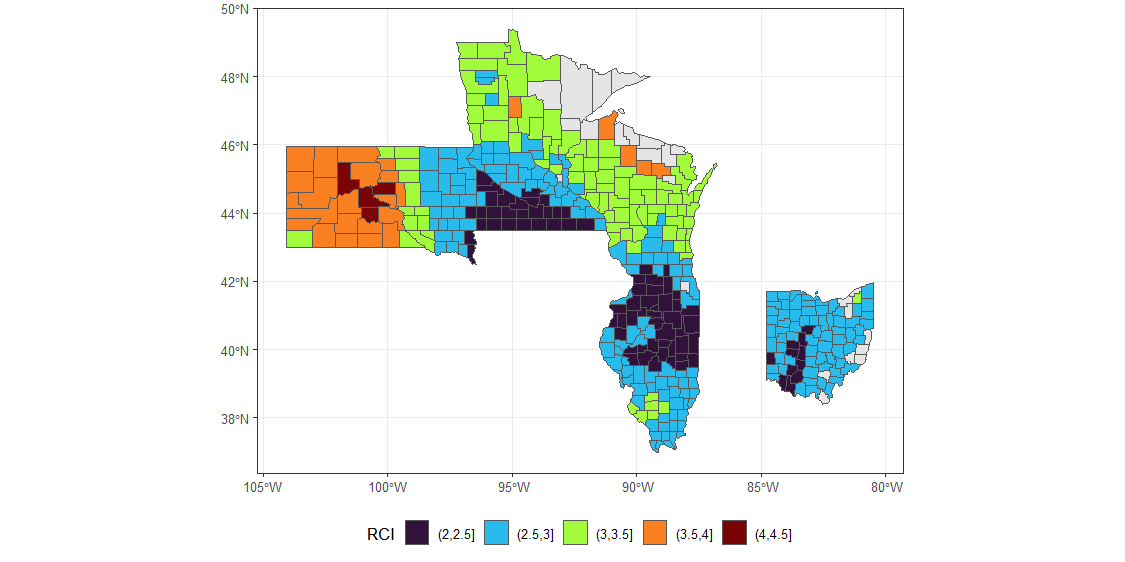
\includegraphics[width=0.85\textwidth]{figures/rci_map}
  \caption{Rotational Complexity Index across Illinois, 2016.}
  \label{fig:rci_map}
  \floatfoot{\footnotesize Notes: Spatial distribution of RCI values computed from
  six-year CDL crop histories at 30-meter resolution. Source: \citet{socolar2021};
  CDL data from USDA-NASS.}
\end{figure}

\subsection{\label{subsec:rot_seq}Crop History, RCI, and Rotation Regimes}
Field-level crop histories come from the USDA Cropland Data Layer \citep[CDL;][]{USDA2015}, an annual raster product produced by NASS that classifies each 30-meter pixel into a crop or land-cover category using satellite imagery and agricultural survey reference data. CDL has been available annually since 2008 for the full contiguous United States and since 2002 for Illinois. We use annual CDL data for Illinois from 2002 to 2022. The corn yield panel runs from 2008 to 2022 (15 outcome years); CDL classifications for 2002 to 2007 enter the analysis only as inputs to the six-year rotation histories of the earliest outcome years, so every outcome year has a complete six-year window.

For each field-pixel and outcome year $t$, we construct a six-year rolling rotation sequence by recording the CDL-classified crop in each of the years $t-1$ through $t-6$, and compute the RCI of \citet{socolar2021} (Section~\ref{subsec:rci}) from that sequence. For the factor-RCI analysis (Sections~\ref{subsec:rci_effects} and~\ref{subsec:rci_vpd_effects}), we apply the same restrictions used to build the sequence-dummy sample in the companion paper: corn is the outcome crop in year $t$; the six-year history contains only corn, soybean, or winter wheat; the field appears in at least two consecutive years in the panel after singleton removal; and the sequence is one of the 29 distinct six-year sequences that together account for approximately 99\% of qualifying field-years. This yields the same common estimation sample of 1,785,861 field-year observations used for the sequence-level results.

For the rotation-regime analysis (Section~\ref{subsec:regimes}), we relax the 99\%-frequency restriction and classify every corn field-year with a non-missing RCI (and non-missing controls and yield) into one of six mutually exclusive regimes: corn monoculture; the perfect alternating corn-soybean rotation; other corn-soybean rotations; corn-soybean rotations that also contain a cereal (winter wheat, another small grain, or sorghum, including their double-crop combinations); corn rotations that contain a forage or specialty crop (alfalfa, hay, clover, or a minor row crop); and corn rotations that contain a year of fallow or pasture. The last two regimes come from splitting the residual ``other crop'' category used in earlier drafts of this analysis: roughly 89\% of that category was grassland, pasture, or fallow and idle cropland, that is, land taken out of active production rather than a diversified rotation, so we separate it from genuine forage and specialty rotations. Precedence runs forage and specialty crops before fallow and pasture, because establishment-year and dormant-year alfalfa stands are frequently coded as pasture in the CDL. Relaxing the 99\%-frequency restriction admits substantially more field-years than the sequence-dummy and factor-RCI samples, including those in the forage, specialty, and fallow-or-pasture regimes that the 29-sequence set excludes by construction; the regime sample comprises 2,288,053 corn field-years.

\subsection{\label{subsec:w_controls}Weather Controls}
We derive monthly precipitation totals, vapor pressure deficit (VPD), and a soil moisture index from GRIDMET \citep{Abatzoglou2013}, available at approximately 4-km spatial resolution. We aggregate each variable to monthly totals or means for June, July, and August. Following \citet{SchlenkerRoberts2009}, we replace monthly mean temperature with growing degree days (GDD) accumulated between 8\textdegree C and 29\textdegree C, and extreme degree days (EDD) accumulated above 29\textdegree C. Climate water deficit data come from TerraClimate \citep{Abatzoglou2018}. For the spatial-lag-of-X specification (Section~\ref{subsec:regimes}), we additionally compute, for each field, the average of the weather and soil vector over its ten nearest neighboring field centroids in an equal-area projection.

\subsection{\label{subsec:soil_controls}Soil Controls}
Soil characteristics come from gSSURGO, produced by the USDA Natural Resources Conservation Service at 30-meter resolution. We extract three field-level measures: the National Commodity Crop Productivity Index (NCCPI), root-zone available water storage (AWC), and soil organic carbon stock (SOC) in the 0-100-centimeter depth zone. For the factor-RCI models, which include field fixed effects, these time-invariant measures are absorbed by the fixed effects and dropped from the preferred specification. For the regime/SLX models, which condition on county rather than field fixed effects, NCCPI and SOC are separately identified and are used as land-quality controls in Section~\ref{subsec:regimes}.

\subsection{\label{subsec:smaple_const}Sample Construction and Summary Statistics}
We construct the estimation sample by merging the QDANN yield raster with CDL rotation sequences and RCI values, GRIDMET and TerraClimate weather covariates, and gSSURGO soil variables at the 30-meter pixel level. The factor-RCI sample comprises the same 1,785,861 field-year observations as the sequence-dummy sample in the companion paper; the regime/SLX sample comprises 2,288,053 field-years.

\begin{table}[!h]
\centering
\caption{\label{tab:corn_summary}Summary statistics by rotation type}
\centering
\resizebox{\ifdim\width>\linewidth\linewidth\else\width\fi}{!}{
\begin{tabular}[t]{lrrrrrrrr}
\toprule
Rotation type & N & Corn yield & RCI & Precip (Jun) & GDD (Jul) & EDD (Jul) & VPD (Jul) & AWC (mm)\\
\midrule
Corn monoculture & 154570 & 187.2 (33.2) & 0.00 (0.00) & 140.9 (70.2) & 409 (52) & 268.3 (2.8) & 1.19 (0.73) & 254 (46)\\
Perfect rotation & 996527 & 194.2 (31.1) & 2.24 (0.00) & 137.0 (67.4) & 420 (43) & 268.4 (2.2) & 1.05 (0.55) & 241 (45)\\
Transitioning & 287280 & 186.3 (33.5) & 1.82 (0.21) & 138.1 (67.8) & 412 (51) & 268.3 (2.7) & 1.16 (0.68) & 250 (45)\\
\bottomrule
\end{tabular}}
\end{table}

\vspace{-1ex}
\noindent{\footnotesize Notes: Means and standard deviations (in parentheses)
for QDANN corn yields and key covariates, by rotation type. Corn monoculture
= C-C-C-C-C-C; Perfect rotation = alternating C-S sequence; Transitioning =
sequences with RCI between 1.41 and 2.00.\par}

Table~\ref{tab:corn_summary} reports summary statistics for three illustrative rotation-type buckets within the factor-RCI corn sample (monoculture, the perfect alternating rotation, and transitioning sequences with RCI between 1.41 and 2.00). The perfect rotation bucket has both the highest mean yield (194.2 bu/acre) and the lowest yield standard deviation (31.1) of the three groups, while continuous corn has the lowest mean yield (187.2) and, together with the transitioning bucket, the highest variability (33.2 and 33.5, respectively); notably, the transitioning bucket -- fields with intermediate RCI values -- does not sit between the other two on either moment, an early signal of the non-monotonicity documented formally in Section~\ref{subsec:rci_effects}.

\section{Econometric Framework\label{sec:econ_framework}}

\subsection{\label{subsec:just_pope}The Just-Pope Framework}
We follow the stochastic production framework of \citet{Just1978, Just1979}:
\begin{equation}
    y = f(\mathbf{X},\alpha)+\sqrt{h(\mathbf{X},\beta)}\times \varepsilon,
\end{equation}
where $f(\cdot)$ is the conditional mean function and $h(\cdot)$ is the conditional variance function, both functions of the same input vector $\mathbf{X}$. This formulation allows any input, including rotational complexity, to raise or lower yield variance independently of its effect on the mean. As in the companion paper, we implement a three-stage FGLS estimator following \citet{Harvey1976} and \citet{Saha1997}, embedded in a panel fixed effects framework with two-way clustering for inference, applied here to factor RCI rather than to individual sequence indicators.

\subsection{\label{subsec:stage_1}Conditional Mean and Variance: Factor-RCI Specification}
We model the conditional mean of corn yields as:
\begin{equation}
    y_{it}=\text{RCI}_{it}'\tau+ W_{it}'\beta+\lambda_{i}+\gamma_{t}+\varepsilon_{it}\label{eq:stage1}
\end{equation}
where $y_{it}$ is the yield of field $i$ year $t$ measured in bushels per acre; $\text{RCI}_{it}$ is a vector of factor RCI indicators, with corn monoculture (RCI $=0$) as the reference category; $W_{it}$ is a vector of weather and soil controls described in Section~\ref{subsec:w_controls}; $\lambda_{i}$ is a field ($\text{tile\_field\_ID}$) fixed effect; and $\gamma_{t}$ is a year fixed effect. Field fixed effects absorb time-invariant field characteristics, and year fixed effects absorb common annual shocks, so identification of $\hat{\tau}$ comes from within-field variation in RCI over time. Standard errors are clustered two-way at the county and year levels, following \cite{Cameron2015}.

To separately identify the effect of RCI on yield risk, we estimate a second-stage regression of squared first-stage residuals on the same regressors:
\begin{equation}
    \hat{u}_{it}^2 = \text{RCI}_{it}'\pi + W_{it}'\delta + \lambda_i + \gamma_t + \nu_{it}\label{eq:stage2}
\end{equation}
where $\hat{u}_{it} = y_{it}-\hat{y}_{it}$ is the stage-1 residual. As in the sequence-level analysis, we treat each observed positive RCI value as a separate indicator rather than imposing a linear functional form, since the central empirical question is precisely whether the RCI-yield relationship is well approximated by a line.

\subsection{\label{subsec:regimes_model}Rotation Regimes and the Spatial-Lag-of-X Model}
The factor-RCI specification lets the data choose the shape of the RCI-yield relationship but still treats RCI as the only summary of rotation history available. As a complementary and more structural approach, we classify each corn field-year's six-year window into one of the six mutually exclusive rotation regimes described in Section~\ref{subsec:rot_seq} and ask whether RCI carries yield information once regime membership is held fixed.

We estimate the regime effects with a spatial-lag-of-X (SLX) specification \citep{HalleckVega2015, LeSagePace2009, Elhorst2014}:
%
\begin{equation}
  y_{it} = \text{regime}_{it}'\theta + W_{it}'\beta + \bar W_{it}'\xi
  + \lambda_k + \gamma_t + \varepsilon_{it}
  \label{eq:slx}
\end{equation}
%
where $\text{regime}_{it}$ is a vector of five regime indicators with corn monoculture omitted, $W_{it}$ is the own-field weather and soil vector of Section~\ref{subsec:w_controls}, and $\bar W_{it}$ is the average of that vector over field $i$'s ten nearest neighbors, computed from field centroids in an equal-area projection. Rotation enters own-field only; only the weather and soil terms are spatially lagged, so $\xi$ captures cross-field growing-condition spillovers rather than a yield-on-yield feedback. We include county and year fixed effects, and we cluster standard errors at 25\,km spatial grid cells. We fix the spatial autoregressive parameter at zero, consistent with the case for SLX over higher-order spatial models when the objects of interest are covariate effects rather than a global yield-on-yield feedback \citep{GibbonsOverman2012}: a lag-in-yield model returned an autoregressive coefficient near zero, freeing it in a spatial Durbin specification produced an inadmissible estimate on a weak instrument set, and the within-year residuals show no spatial autocorrelation (Moran's $I$ on the SLX residuals, computed year by year against the same ten-nearest-neighbor weights, averages 0.016 across 15 years and is never significant at the 5\% level), so a spatial HAC correction in the manner of \citet{Conley1999} is unnecessary and clustered SLX standard errors are adequate. This specification is estimated on 2,288,053 corn field-years, more than the factor-RCI sample of Sections~\ref{subsec:stage_1} and~\ref{subsec:rci_effects}. The difference is one of sample definition: the regime sample retains every corn field-year with a non-missing RCI, whereas the factor-RCI sample further restricts to the 29 six-year sequences that clear the 99\% support threshold. Relaxing that restriction is what admits the additional field-years here, including those in the forage, specialty, and fallow-or-pasture regimes that the 29-sequence set excludes by construction.

Equation~\eqref{eq:slx} conditions on county rather than field fixed effects, because regime is close to time-invariant for most fields in the panel and would be poorly identified off of within-field switches alone; this also means that field-level, time-invariant land-quality measures such as NCCPI and soil organic carbon are separately identified here (unlike in the field-fixed-effects factor-RCI model), which we exploit directly as a land-quality-sorting check in Section~\ref{subsec:regimes}.

\section{\label{sec:results}Results}

\subsection{\label{subsec:rci_effects}Rotational Complexity Index Effects}


\begin{table}[H]
   \caption{\label{tab:corn_rci} Rotation Complexity and corn yields}
   \bigskip
   \centering
   \begin{tabular}{lcc}
      \toprule
       & \multicolumn{2}{c}{corn\_yield}\\
                                      & No controls             & Weather and soil controls \\   
                                      & (1)                     & (2)\\  
      \midrule 
      RCI = 1.41                      & 0.4057 (0.8041)         & 0.6237 (0.7213)\\   
      RCI = 1.73                      & -2.035$^{***}$ (0.6712) & -2.037$^{***}$ (0.6014)\\   
      RCI = 2                         & 0.0377 (0.5986)         & -0.5767 (0.5867)\\   
      RCI = 2.24                      & 0.5905 (0.6741)         & -0.5664 (0.6785)\\   
      RCI = 2.45                      & 0.6316 (0.7670)         & -0.1331 (0.7103)\\   
      RCI = 2.65                      & 1.751$^{**}$ (0.7580)   & 0.6746 (0.7601)\\   
      RCI = 2.74                      & -1.520 (1.273)          & 2.421$^{**}$ (1.215)\\   
      RCI = 3                         & 1.204 (1.348)           & -0.1339 (1.126)\\   
      RCI = 3.24                      & 5.085$^{***}$ (1.126)   & 1.733$^{*}$ (0.9865)\\   
      RCI = 3.46                      & 11.91$^{***}$ (1.481)   & 3.963$^{***}$ (1.509)\\   
      RCI = 3.74                      & 10.60$^{***}$ (1.775)   & 3.860$^{**}$ (1.581)\\   
      RCI = 4                         & 15.65$^{***}$ (1.926)   & 7.844$^{***}$ (1.931)\\   
       \\
      Observations                    & 1,581,271               & 1,581,271\\  
      R$^2$                           & 0.81129                 & 0.83643\\  
      Within R$^2$                    & 0.00408                 & 0.13675\\  
       \\
      tile\_field\_ID fixed effects   & $\checkmark$            & $\checkmark$\\   
      year fixed effects              & $\checkmark$            & $\checkmark$\\   
      \bottomrule
   \end{tabular}
\end{table}



\begin{quote}
\small
Notes: RCI entered as a factor variable; reference category is RCI = 0 (corn monoculture). Column (1) excludes weather and soil controls; column (2) includes the full control vector. Field (tile\_field\_ID) and year fixed effects are included in both columns; standard errors are two-way clustered at county and year.
\end{quote}

\begin{figure}[H]
  \centering
  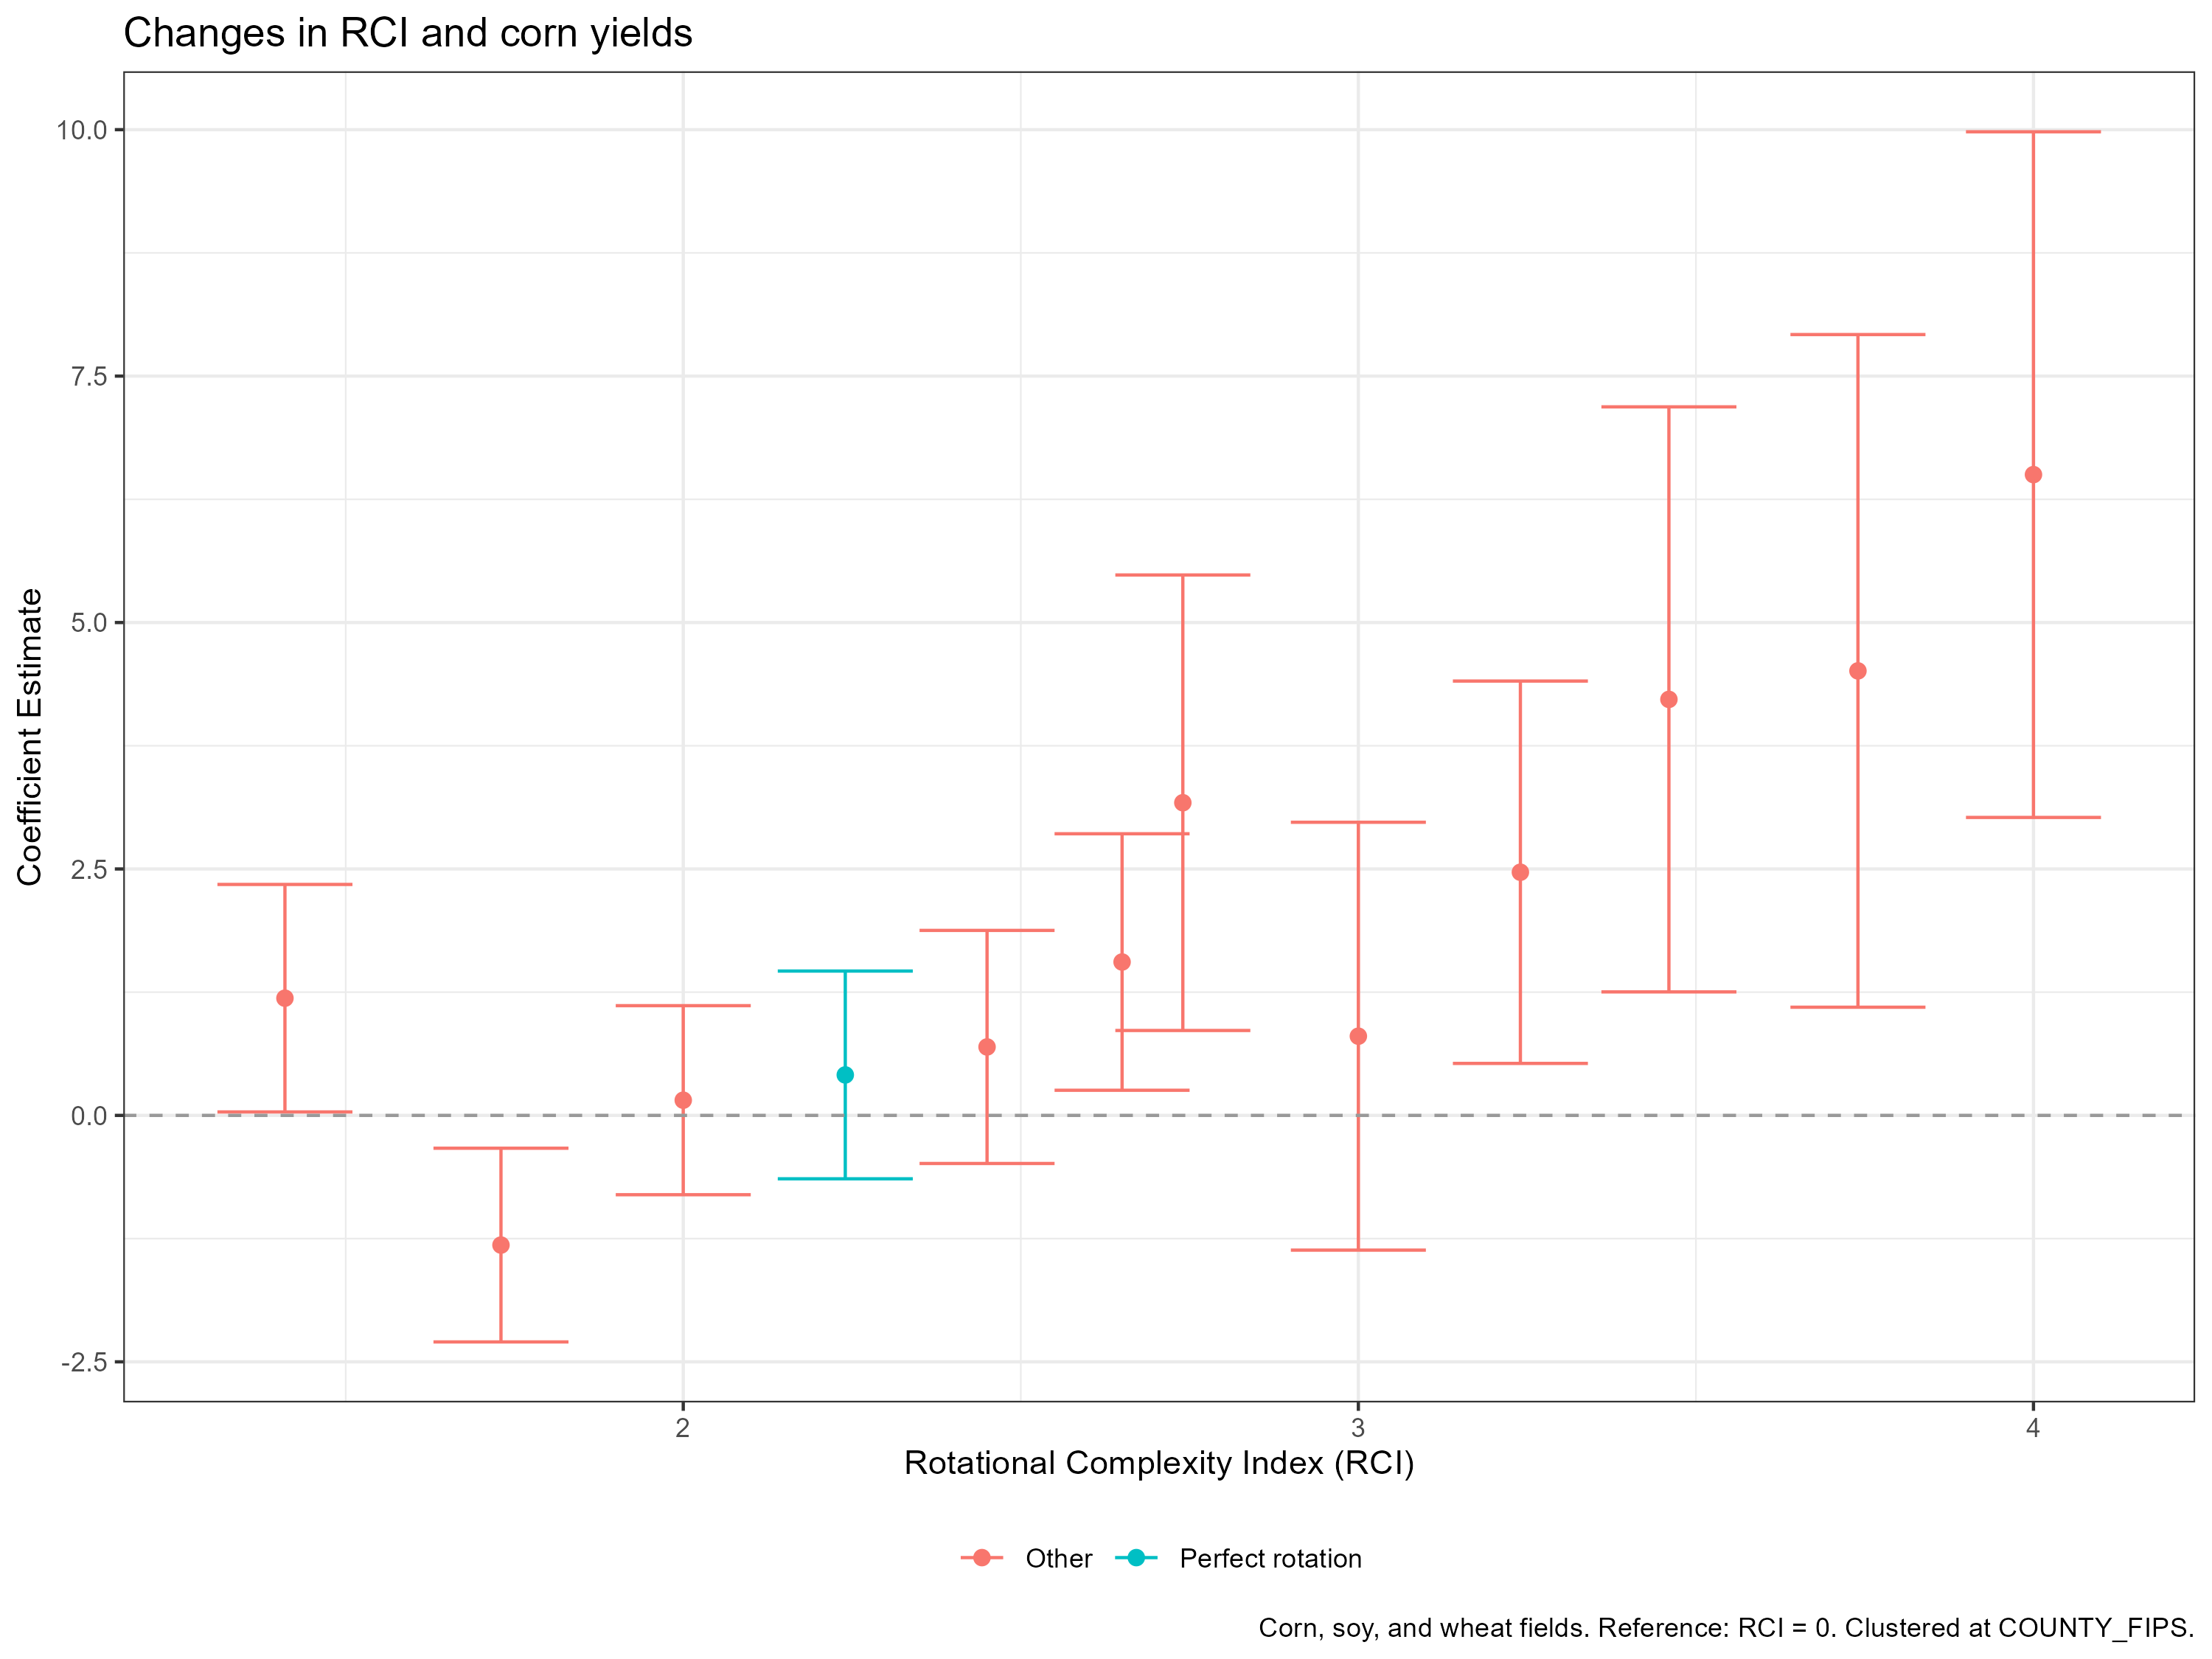
\includegraphics[width=\textwidth]{figures/corn_rci_plot}
  \caption{Nonlinear effect of RCI on corn yield mean and variance.}
  \label{fig:corn_rci_plot}
  \floatfoot{\footnotesize Notes: Factor RCI coefficients from
  equation~\eqref{eq:stage1} (mean, left panel) and equation~\eqref{eq:stage2}
  (variance, right panel), on corn fields with corn, soybean, and winter-wheat
  rotation histories. Shaded
  area is the 95\% confidence interval. Reference: RCI = 0 (corn monoculture).
  Two-way clustering at county and year level.}
\end{figure}

Table~\ref{tab:corn_rci} and Figure~\ref{fig:corn_rci_plot} report the effects of factor RCI on corn yields, jointly for the mean and variance equations. Every RCI level above the corn-monoculture reference carries a positive and statistically significant mean coefficient, but the effect is not monotonic in RCI. Relative to monoculture (column 2, full controls), the mean premium rises to about 2.0 bushels per acre at RCI = 1.73, falls to 1.3 at RCI = 2.00, climbs to roughly 4.0 at RCI = 2.45, drops back to 3.1 at RCI = 2.65, and peaks near 5.9 at RCI = 3.00 before declining again across the two highest levels (5.3 at RCI = 3.24 and 4.8 at RCI = 3.46). Adjacent RCI values thus differ by one to three bushels per acre in either direction, and the premium peaks in the middle of the observed range rather than at its top. The mapping from RCI to yield is positive on average but too irregular for a linear premium adjustment to represent.

\subsection{\label{subsec:regimes}Rotation Regimes and the Limits of RCI}

\begin{table}[H]
  \centering
  \caption{Corn yield by rotation regime (SLX specification).}
  \label{tab:slx_corn_regime}
  
\begingroup
\centering
\begin{tabular}{lc}
   \tabularnewline \midrule \midrule
   Dependent Variable:     & corn\_yield\\   
   Model:                  & (1)\\  
   \midrule
   \emph{Variables}\\
   corn\_soy\_perfect      & 2.371$^{***}$\\   
                           & (0.2602)\\   
   corn\_soy\_other        & 0.5325$^{**}$\\   
                           & (0.2420)\\   
   corn\_soy\_cereal       & -0.9645$^{***}$\\   
                           & (0.2930)\\   
   corn\_other\_crops      & -5.482$^{***}$\\   
                           & (0.6183)\\   
   corn\_fallow\_pasture   & -6.659$^{***}$\\   
                           & (0.3293)\\   
   \midrule
   \emph{Fixed-effects}\\
   COUNTY\_FIPS            & Yes\\  
   year                    & Yes\\  
   \midrule
   \emph{Fit statistics}\\
   Observations            & 2,288,053\\  
   R$^2$                   & 0.76166\\  
   Within R$^2$            & 0.15337\\  
   \midrule \midrule
   \multicolumn{2}{l}{\emph{Clustered (grid\_cell) standard-errors in parentheses}}\\
   \multicolumn{2}{l}{\emph{Signif. Codes: ***: 0.01, **: 0.05, *: 0.1}}\\
\end{tabular}
\par\endgroup



\end{table}
\begin{quote}
\small
Notes: Estimates of equation~\eqref{eq:slx}. The dependent variable is corn yield in bushels per acre. Regime indicators are relative to corn monoculture. We include own-field weather and soil covariates and their spatial lags but suppress them from the display. County and year fixed effects are included. We cluster standard errors at the 25\,km spatial grid cell level.
\end{quote}

Table~\ref{tab:slx_corn_regime} reports the regime effects. Relative to corn monoculture, the perfect alternating corn-soybean rotation raises yield by about 2.4 bushels per acre and other corn-soybean rotations by about 0.5. In contrast, the three regimes that leave the corn-soybean system carry large negative coefficients: about $-1.0$ bushels per acre for corn-soybean-cereal, $-5.5$ for corn rotations containing a forage or specialty crop, and $-6.7$ for corn rotations containing a fallow or pasture year. All five coefficients are significant at the 1\% level except other corn-soybean rotations, which is significant at 5\%. The ordering matches the sequence-level results reported in the companion paper: diversification within the corn-soybean system helps, whereas a year of idled or perennial land in the window coincides with a sharp yield deficit, consistent with those regimes capturing land taken out of intensive production rather than a deliberate rotation. The spatially-lagged weather and soil terms absorb cross-field growing-condition spillovers so they do not contaminate the regime coefficients; their estimates are of no independent interest here and are suppressed from the display. Rotation enters own-field only and is not spatially lagged, so the regime coefficients in Table~\ref{tab:slx_corn_regime} are the total regime effect.

Table~\ref{tab:slx_corn_regime_gaps} reports all fifteen pairwise contrasts between regimes, with delta-method standard errors. Every contrast is significant, but the magnitudes fall into two groups. The perfect and other corn-soybean regimes sit six to nine bushels per acre above the forage, specialty, and fallow or pasture regimes, and every one of those boundary-spanning contrasts is significant at the 1\% level. The contrasts within the corn-soybean system are several times smaller, ranging from about half a bushel (monoculture versus other corn-soybean) to about 3.3 bushels (perfect corn-soybean versus corn-soybean-cereal).

\begin{table}[H]
  \centering
  \caption{Pairwise yield gaps between rotation regimes.}
  \label{tab:slx_corn_regime_gaps}
  
\begingroup
\centering
\begin{tabular}{lc}
   \tabularnewline \midrule \midrule
   Contrast & Difference (bu/acre)\\
   \midrule
   Perfect corn-soybean $-$ Corn + fallow/pasture & 9.030$^{***}$\\
   & (0.307)\\
   Perfect corn-soybean $-$ Corn + forage/specialty & 7.853$^{***}$\\
   & (0.617)\\
   Other corn-soybean $-$ Corn + fallow/pasture & 7.191$^{***}$\\
   & (0.284)\\
   Corn monoculture $-$ Corn + fallow/pasture & 6.659$^{***}$\\
   & (0.329)\\
   Other corn-soybean $-$ Corn + forage/specialty & 6.015$^{***}$\\
   & (0.603)\\
   Corn-soybean-cereal $-$ Corn + fallow/pasture & 5.694$^{***}$\\
   & (0.258)\\
   Corn monoculture $-$ Corn + forage/specialty & 5.482$^{***}$\\
   & (0.618)\\
   Corn-soybean-cereal $-$ Corn + forage/specialty & 4.518$^{***}$\\
   & (0.640)\\
   Perfect corn-soybean $-$ Corn-soybean-cereal & 3.335$^{***}$\\
   & (0.219)\\
   Corn monoculture $-$ Perfect corn-soybean & -2.371$^{***}$\\
   & (0.260)\\
   Perfect corn-soybean $-$ Other corn-soybean & 1.839$^{***}$\\
   & (0.113)\\
   Other corn-soybean $-$ Corn-soybean-cereal & 1.497$^{***}$\\
   & (0.227)\\
   Corn + forage/specialty $-$ Corn + fallow/pasture & 1.176$^{*}$\\
   & (0.664)\\
   Corn monoculture $-$ Corn-soybean-cereal & 0.964$^{***}$\\
   & (0.293)\\
   Corn monoculture $-$ Other corn-soybean & -0.532$^{**}$\\
   & (0.242)\\
   \midrule \midrule
   \multicolumn{2}{l}{\emph{Delta-method standard errors, 25\,km grid-cell clustered, in parentheses}}\\
   \multicolumn{2}{l}{\emph{Signif. Codes: ***: 0.01, **: 0.05, *: 0.1}}\\
\end{tabular}
\par\endgroup


\end{table}
\begin{quote}
\small
Notes: Each row is the difference in the regime coefficient of equation~\eqref{eq:slx} between the two named regimes (positive means the first regime yields more), with corn monoculture normalized to zero. Rows are ordered by absolute gap. Delta-method standard errors, clustered on 25\,km spatial grid cells, in parentheses.
\end{quote}

A natural concern is that the regime ranking reflects land-quality sorting: fields on better soil may both yield more and be more likely to carry a diversified rotation. Because equation~\eqref{eq:slx} conditions on county and year fixed effects rather than field fixed effects, field-level soil measures are identified here and can be entered directly. Table~\ref{tab:slx_corn_regime_ctrl} re-estimates the regime model with the National Commodity Crop Productivity Index for corn and the soil organic carbon stock added as controls. The regime coefficients barely move: the two corn-soybean coefficients change by less than 0.01 bushel per acre, corn-soybean-cereal by about 0.01, and the two idled-land regimes attenuate only modestly (corn-plus-forage from $-5.48$ to $-5.24$, corn-plus-fallow from $-6.66$ to $-5.80$) while remaining large and significant at the 1\% level. The regime ranking is therefore not an artifact of land-quality sorting; fields carrying diversified rotations are not simply the fields on better soil.

\begin{table}[H]
  \centering
  \caption{Regime model with and without land-quality controls.}
  \label{tab:slx_corn_regime_ctrl}
  
\begingroup
\centering
\begin{tabular}{lcc}
   \tabularnewline \midrule \midrule
   Dependent Variable: & \multicolumn{2}{c}{corn\_yield}\\
                           & baseline        & + land-quality controls \\   
   Model:                  & (1)             & (2)\\  
   \midrule
   \emph{Variables}\\
   corn\_soy\_perfect      & 2.371$^{***}$   & 2.290$^{***}$\\   
                           & (0.2602)        & (0.2527)\\   
   corn\_soy\_other        & 0.5325$^{**}$   & 0.5374$^{**}$\\   
                           & (0.2420)        & (0.2392)\\   
   corn\_soy\_cereal       & -0.9645$^{***}$ & -0.9756$^{***}$\\   
                           & (0.2930)        & (0.2813)\\   
   corn\_other\_crops      & -5.482$^{***}$  & -5.242$^{***}$\\   
                           & (0.6183)        & (0.6563)\\   
   corn\_fallow\_pasture   & -6.659$^{***}$  & -5.802$^{***}$\\   
                           & (0.3293)        & (0.3364)\\   
   \midrule
   \emph{Fixed-effects}\\
   COUNTY\_FIPS            & Yes             & Yes\\  
   year                    & Yes             & Yes\\  
   \midrule
   \emph{Fit statistics}\\
   Observations            & 2,288,053       & 2,288,053\\  
   R$^2$                   & 0.76166         & 0.76636\\  
   Within R$^2$            & 0.15337         & 0.17009\\  
   \midrule \midrule
   \multicolumn{3}{l}{\emph{Clustered (grid\_cell) standard-errors in parentheses}}\\
   \multicolumn{3}{l}{\emph{Signif. Codes: ***: 0.01, **: 0.05, *: 0.1}}\\
\end{tabular}
\par\endgroup



\end{table}
\begin{quote}
\small
Notes: Column (1) repeats the regime-only model of
Table~\ref{tab:slx_corn_regime}. Column (2) adds the field-level National
Commodity Crop Productivity Index for corn and the 0-100\,cm soil organic carbon
stock (Section~\ref{subsec:soil_controls}). Both soil measures are time-invariant
and would be absorbed by field fixed effects, but are identified here because
equation~\eqref{eq:slx} conditions on county and year effects only. County and year fixed effects are
included. Standard errors are clustered at the 25\,km spatial grid cell level.
\end{quote}

Conditional on regime, RCI adds nothing that is separately identified. Within each regime, RCI takes only 15 to 18 distinct values with a standard deviation between 0.33 and 0.68, so it is close to constant. A hybrid model that keeps the regime levels and adds a regime-specific RCI slope is degenerate for two independent reasons. First, the near-constant within-regime RCI makes each regime-level indicator and its regime-specific RCI slope nearly linearly dependent: regime-level standard errors inflate from 0.24 to 0.61 in the regime-only model to about 51 in the hybrid, while the slopes appear tightly estimated. The sum of the level and slope terms is identified, but the split between them is not. Second, the interaction term is undefined for the two regimes in which RCI never varies (corn monoculture and the perfect alternating rotation), so those field-years drop, and the sample falls from about 2.29 million to about 1.14 million, silently reducing the ``hybrid'' to a four-regime model on half the data. Table~\ref{tab:slx_corn_regime_hybrid} shows the failure for the record; it is not a specification we report as a preferred estimate.

\begin{table}[H]
  \centering
  \caption{Regime-only versus hybrid regime-plus-RCI-slope model.}
  \label{tab:slx_corn_regime_hybrid}
  
\begingroup
\centering
\begin{tabular}{lcc}
   \tabularnewline \midrule \midrule
   Dependent Variable: & \multicolumn{2}{c}{corn\_yield}\\
                                                   & regime-only (REPORTED) & hybrid (DEGENERATE: SE~51, n halved) \\   
   Model:                                          & (1)                    & (2)\\  
   \midrule
   \emph{Variables}\\
   regime\_vcorn\_fallow\_pasture $\times$ RCI     &                        & 2.780$^{***}$\\   
                                                   &                        & (0.2003)\\   
   regime\_vcorn\_other\_crops $\times$ RCI        &                        & -1.210$^{***}$\\   
                                                   &                        & (0.4412)\\   
   regime\_vcorn\_soy\_cereal $\times$ RCI         &                        & 0.5222$^{**}$\\   
                                                   &                        & (0.2648)\\   
   regime\_vcorn\_soy\_other $\times$ RCI          &                        & 0.8287$^{***}$\\   
                                                   &                        & (0.1791)\\   
   \midrule
   \emph{Fixed-effects}\\
   COUNTY\_FIPS                                    & Yes                    & Yes\\  
   year                                            & Yes                    & Yes\\  
   \midrule
   \emph{Fit statistics}\\
   Observations                                    & 2,288,053              & 1,136,956\\  
   R$^2$                                           & 0.76166                & 0.75570\\  
   Within R$^2$                                    & 0.15337                & 0.15956\\  
   \midrule \midrule
   \multicolumn{3}{l}{\emph{Clustered (grid\_cell) standard-errors in parentheses}}\\
   \multicolumn{3}{l}{\emph{Signif. Codes: ***: 0.01, **: 0.05, *: 0.1}}\\
\end{tabular}
\par\endgroup



\end{table}
\begin{quote}
\small
Notes: Column (1) is the regime-only model of Table~\ref{tab:slx_corn_regime}.
Column (2) adds regime-specific RCI slopes for the four regimes in which RCI
varies; its regime-level standard errors reach roughly 51, and its sample is
halved, because the two constant-RCI regimes have no interaction term. The column
(2) RCI slopes are shown only to document the degeneracy and should not be read
as evidence that RCI affects yield within a regime.
\end{quote}

Taken with Section~\ref{subsec:rci_effects}, this sharpens the paper's central point. RCI is not merely non-monotone in yield: once an agronomically meaningful regime describes rotation history, RCI has no separately identified yield effect, and the apparent RCI slopes in interaction models are regime-level yield differences passing through the RCI-regime collinearity. A rotation-conditioned insurance rate should condition on rotation structure -- the regime, or the structural sequence features used in the companion paper -- rather than on a scalar complexity index.

\subsection{\label{subsec:rci_vpd_effects}Rotational Complexity and Drought: Interaction Effects}


\begin{table}[H]
   \caption{\label{tab:corn_rci_vpd} RCI x drought interaction effects on corn yields}
   \bigskip
   \centering
   \begin{tabular}{lc}
      \toprule
                                            & corn\_yield\\   
                                            & (1)\\  
      \midrule 
      RCI1.41                               & -0.7067$^{***}$\\   
                                            & (0.2238)\\   
      RCI1.73                               & 2.055$^{***}$\\   
                                            & (0.2710)\\   
      RCI2                                  & 0.8744$^{***}$\\   
                                            & (0.2479)\\   
      RCI2.24                               & 3.520$^{***}$\\   
                                            & (0.3709)\\   
      RCI2.45                               & 4.025$^{***}$\\   
                                            & (0.3736)\\   
      RCI2.65                               & 3.773$^{***}$\\   
                                            & (0.7362)\\   
      RCI3                                  & 3.996$^{***}$\\   
                                            & (1.029)\\   
      RCI3.24                               & 6.401$^{***}$\\   
                                            & (0.8356)\\   
      RCI3.46                               & 4.655$^{***}$\\   
                                            & (0.7854)\\   
      Somewhat dry season                   & -2.682$^{***}$\\   
                                            & (0.5983)\\   
      Dry season                            & -0.1092\\   
                                            & (1.237)\\   
      RCI1.41 $\times$ Somewhat dry season  & 1.421$^{***}$\\   
                                            & (0.3600)\\   
      RCI1.73 $\times$ Somewhat dry season  & 0.1551\\   
                                            & (0.3170)\\   
      RCI2 $\times$ Somewhat dry season     & 1.611$^{***}$\\   
                                            & (0.3315)\\   
      RCI2.24 $\times$ Somewhat dry season  & 1.582$^{***}$\\   
                                            & (0.5517)\\   
      RCI2.45 $\times$ Somewhat dry season  & 1.868$^{***}$\\   
                                            & (0.4863)\\   
      RCI2.65 $\times$ Somewhat dry season  & 0.7448\\   
                                            & (0.9522)\\   
      RCI3 $\times$ Somewhat dry season     & 1.842\\   
                                            & (1.806)\\   
      RCI3.24 $\times$ Somewhat dry season  & 2.025\\   
                                            & (1.397)\\   
      RCI3.46 $\times$ Somewhat dry season  & 1.154\\   
                                            & (1.393)\\   
      RCI1.41 $\times$ Dry season           & -0.1634\\   
                                            & (0.5432)\\   
      RCI1.73 $\times$ Dry season           & 0.3209\\   
                                            & (0.5124)\\   
      RCI2 $\times$ Dry season              & 0.9056$^{*}$\\   
                                            & (0.5435)\\   
      RCI2.24 $\times$ Dry season           & -2.453$^{***}$\\   
                                            & (0.8526)\\   
      RCI2.45 $\times$ Dry season           & -1.225\\   
                                            & (0.7723)\\   
      RCI2.65 $\times$ Dry season           & -2.368$^{***}$\\   
                                            & (0.8725)\\   
      RCI3 $\times$ Dry season              & 5.359$^{***}$\\   
                                            & (1.807)\\   
      RCI3.24 $\times$ Dry season           & -5.319$^{***}$\\   
                                            & (1.501)\\   
      RCI3.46 $\times$ Dry season           & 0.1165\\   
                                            & (1.604)\\   
       \\
      Observations                          & 1,785,861\\  
      R$^2$                                 & 0.84340\\  
      Within R$^2$                          & 0.15306\\  
       \\
      tile\_field\_ID fixed effects         & $\checkmark$\\   
      year fixed effects                    & $\checkmark$\\   
      \bottomrule
   \end{tabular}
\end{table}



\begin{quote}
\small
Notes: Dependent variable is QDANN corn yield in bushels per acre. RCI enters as
a factor variable interacted with July VPD dry-season bins (\emph{Somewhat dry},
1.9-2.1 kPa; \emph{Dry}, $>$2.1 kPa; normal $<$1.9 kPa omitted). Main effects
and interaction terms are shown. Corn monoculture (RCI = 0) is the omitted RCI
category. Field (\texttt{tile\_field\_ID}) and year fixed effects included;
standard errors two-way clustered at county and year, in parentheses.
$^{***}p<0.01$, $^{**}p<0.05$, $^{*}p<0.10$.
\end{quote}

Table~\ref{tab:corn_rci_vpd} interacts factor RCI with the July drought bins to ask whether more complex rotations buffer corn yields against dry conditions, the field-level analog of the resilience mechanism documented experimentally by \citet{bowles2020}. The evidence is mixed and, as elsewhere in this paper, non-monotone in RCI. Under \emph{somewhat dry} conditions, the interaction terms are predominantly positive, though significant at only two RCI levels (RCI = 1.41 and 2.00), weakly indicating that moderate rotational complexity partially offsets the roughly 2.5 bushel-per-acre penalty of a somewhat dry July. Under \emph{dry} conditions, however, the interactions change sign repeatedly across adjacent RCI levels and are individually imprecise (only one of the nine is even marginally significant), so the table does not support a clean claim that higher RCI buffers corn against severe drought. This pattern reinforces the paper's central message: RCI is too coarse and too non-monotone a summary of rotation structure to carry a stable interaction with weather risk, which is precisely the property that would be required for a linear RCI-based adjustment to crop insurance rates to be correctly specified.

\section{\label{sec:conclusions}Discussion and Conclusions}

\subsection{\label{susec:summary}Summary of Findings}

This paper uses a large satellite-based field-level panel of Illinois corn yields from 2008 to 2022, with rotation histories built from Cropland Data Layer records back to 2002, to evaluate whether the Rotational Complexity Index and a set of mutually exclusive rotation regimes carry usable information about the mean and variance of corn yields, and whether that information interacts with the spatial structure of growing conditions. Our main findings are three.

First, the RCI does not map cleanly onto corn yields. Every observed RCI level above the corn-monoculture reference raises mean yield significantly, but the increments are non-monotone in RCI: the estimated premium moves up and down by one to three bushels per acre between adjacent levels and peaks near RCI $=3.00$ rather than at the top of the range. No linear function of RCI captures this pattern, which is what a linear premium adjustment based on RCI would miss.

Second, once fields are classified into six mutually exclusive rotation regimes, RCI adds no separately identified yield information: RCI is close to constant within regime, and a hybrid model with regime-specific RCI slopes is econometrically degenerate. The regime classification itself is informative, however: diversification within the corn-soybean system raises yields relative to monoculture, while regimes that take land out of active corn-soybean production coincide with yield deficits of five to seven bushels per acre, a pattern that survives controlling for land quality and is not an artifact of land-quality sorting across space.

Third, interactions between RCI and July drought severity are non-monotone and mostly statistically imprecise, offering no stable evidence that rotational complexity buffers corn against drought at the field level, in contrast to the resilience benefits documented in long-term experimental diversification trials.

\subsection{\label{subsec:implications}Implications for Crop Insurance Rating}

Our findings caution against using the RCI, or any single scalar diversity index, as a rotation-conditioning variable in federal crop insurance rating. A linear RCI-based premium adjustment would systematically overcharge fields with high RCI values that feature agronomically suboptimal sequencing, and undercharge fields with moderate RCI values that nonetheless achieve strong yield outcomes. Even a nonlinear, factor-RCI adjustment would be redundant once rotation regime is accounted for, since RCI carries no separately identified information conditional on regime. A companion paper shows that a small set of structural features describing the timing and spacing of soybean placement within the rotation window predicts yield outcomes more informatively, and proposes a rotation score built from those features as a concrete, field-computable alternative rating input.

The regime results additionally suggest that any rotation-conditioned rate should distinguish diversification within the corn-soybean system from regimes that idle land or introduce a perennial or specialty crop, since these two categories of rotation have opposite-signed and economically large effects on yield that a scalar index conflates.

\subsection{\label{subsec:limitations}Limitations and Future Work}

Our analysis has several limitations. First, the yield data come from a satellite-based estimator (QDANN) with a meaningful field-level error rate, and, following \citet{Benami2026}, this measurement error need not be classical. If QDANN's prediction error is uncorrelated with rotation history, it behaves as classical measurement error and attenuates our estimates toward zero. If, however, QDANN's accuracy varies systematically with field characteristics that are themselves correlated with rotation choice, the resulting non-classical measurement error could bias our estimates in either direction, not only toward zero. We do not have the tools to rule out this possibility here and flag it as a first-order concern for future work using EO-derived yield products for rotation-effect estimation.

Second, the regime and SLX specifications condition on county rather than field fixed effects, so identification relies more heavily on cross-field comparisons within a county-year than the field-fixed-effects sequence and factor-RCI models do. We address the most obvious threat, land-quality sorting, directly in Table~\ref{tab:slx_corn_regime_ctrl}, but residual selection on unobserved, time-invariant field characteristics correlated with regime choice cannot be fully ruled out with county rather than field fixed effects.

Third, our analysis covers corn rotations involving soybean and winter wheat in Illinois, with a residual forage/specialty and fallow/pasture category that is coarser than a full agronomic classification would allow; generalizability to other Corn Belt states and to different climate and soil regimes is an open question. Finally, rotation decisions respond endogenously to prices and the proximity of grain market infrastructure such as ethanol refineries \citep{Pates2025,cheu2025}, which is a further reason the spatial pattern of rotation choice documented here should not be read as fully exogenous to yield outcomes.

\section{\label{sec:conclusion}Conclusion}

This paper shows that the Rotational Complexity Index, despite its standing as the field-scale measure of rotational diversity in the Corn Belt literature, is not a suitable input for rotation-conditioned crop insurance rating. The RCI moves non-monotonically with corn yields across its observed range, and once rotation history is instead summarized through a small number of mutually exclusive regimes, RCI adds no separately identified information: a hybrid model combining regime and RCI is econometrically degenerate. The regime classification is itself informative -- diversification within the corn-soybean system raises yields, while regimes that idle land or introduce a perennial or specialty crop carry large yield penalties that survive controlling for land quality -- but that information comes from the regime categories, not from RCI as a scalar summary. Interactions between RCI and drought severity are similarly non-monotone and imprecise, offering no stable evidence of a complexity-driven drought buffer at the field level.

Two qualifications bound how far these findings can be pushed toward an actual rating change. First, we document effects in bushels per acre, not in premium dollars: converting these magnitudes into a rate adjustment, and checking that adjustment against the cross-subsidization concerns raised by \citet{Ramaswami1993} and \citet{Babcock1996}, is necessary before any of this could inform an actual RMA rate filing. Second, our identification comes from a single state and a sample dominated by corn-soybean rotations; whether the RCI's non-monotonicity and the regime ordering documented here hold more broadly for other Corn Belt geographies is untested here. A companion paper takes the constructive next step, using the same field-level pipeline to build and validate a rotation score from structural sequence features that does not share RCI's shortcomings.

\newpage
\bibliography{bibliography.bib}

\newpage
\ Appendix

\section*{Tables}


\begin{table}[H]
   \caption{\label{tab:corn_rci_jp} Just-Pope: factor RCI and corn yield moments}
   \bigskip
   \centering
   \begin{tabular}{lcc}
      \toprule
                                      & corn\_yield          & resid\_sq\\   
                                      & Mean                 & Variance \\   
                                      & (1)                  & (2)\\  
      \midrule 
      RCI = 1.41                      & 0.1133 (1.278)       & -8.801 (10.23)\\   
      RCI = 1.73                      & -2.336 (1.590)       & 5.031 (17.63)\\   
      RCI = 2                         & -0.4267 (1.118)      & 1.148 (8.530)\\   
      RCI = 2.24                      & -0.5367 (1.376)      & 1.222 (8.965)\\   
      RCI = 2.45                      & -0.0163 (1.316)      & 4.833 (10.09)\\   
      RCI = 2.65                      & 0.7787 (1.371)       & -1.980 (9.868)\\   
      RCI = 2.74                      & 2.080 (1.744)        & -15.34 (15.15)\\   
      RCI = 3                         & -0.3399 (1.900)      & -30.51 (23.78)\\   
      RCI = 3.24                      & 1.538 (1.920)        & -36.69 (22.12)\\   
      RCI = 3.46                      & 3.957 (3.199)        & -44.62 (35.92)\\   
      RCI = 3.74                      & 3.764 (2.644)        & -64.85$^{*}$ (31.69)\\   
      RCI = 4                         & 7.918$^{**}$ (2.993) & -58.09 (38.90)\\   
       \\
      Observations                    & 1,640,455            & 1,640,455\\  
      R$^2$                           & 0.83737              & 0.30092\\  
      Within R$^2$                    & 0.13850              & 0.01313\\  
       \\
      tile\_field\_ID fixed effects   & $\checkmark$         & $\checkmark$\\   
      year fixed effects              & $\checkmark$         & $\checkmark$\\   
      \bottomrule
   \end{tabular}
\end{table}



\begin{quote}
\small
Notes: Column (1) reports stage-1 mean coefficients; column (2) reports stage-2 OLS variance coefficients. Reference: RCI = 0 (corn monoculture). Field (tile\_field\_ID) and year fixed effects included; two-way clustering at county and year level.
\end{quote}

\end{document}
